\documentclass[11pt]{book}
\usepackage[bg-letter]{lib/rpg-book} % Options: bg-a4, bg-letter, bg-full, bg-print, bg-none.
\usepackage[english]{babel}
\usepackage[utf8]{inputenc}
\usepackage[hidelinks]{hyperref}

\usepackage[T1]{fontenc}
\usepackage{tgcursor}
\usepackage{xcolor}
\usepackage{soul}
\usepackage{enumitem}
\usepackage{wrapfig}
\usepackage{caption}
\usepackage{subcaption}
\usepackage{float}
\usepackage{multicol}
\usepackage{rotating}
\usepackage{tikz}
\usepackage{wrapfig}
\usepackage{lettrine}
\usepackage{aurical}
\usepackage{pgothic}

\renewcommand{\LettrineTextFont}{\normalfont}
\renewcommand{\LettrineFontHook}{\pgothfamily}

\makeatletter
\newcommand{\globalcolor}[1]{%
  \color{#1}\global\let\default@color\current@color
}
\makeatother

\makeatletter
\def\newsect{%
    \vskip2em plus0.5em minus0.5em%
    \hbox to\linewidth{\hfil*\quad\quad*\quad\quad*\hfil}%
    \penalty10000\vskip2em plus0.5em minus0.5em%
    \@afterindentfalse\@afterheading%
}
\makeatother%


\newcommand\blfootnote[1]{%
  \begingroup
  \renewcommand\thefootnote{}\footnote{#1}%
  \addtocounter{footnote}{-1}%
  \endgroup
}


\definecolor{alien}{HTML}{660f00}

\definecolor{PC}{HTML}{c0ccc1}

\definecolor{lightgray}{gray}{0.9}
% \sethlcolor{lightgray}


\newcommand\pc[1]{\colorbox{PC}{\color{black} #1}}

% https://tex.stackexchange.com/questions/12262/multicol-and-figures
\newenvironment{Figure}
  {\par\medskip\noindent\minipage{\linewidth}}
  {\endminipage\par\medskip}
%  

% \AtBeginDocument{\globalcolor{alien}}as

\title{Old Epic}
\date{\today}
\author{Arthur Marques}





% Start document
\begin{document}
\fontfamily{ppl}\selectfont % Set text font
\frontmatter

% \maketitle



% \tableofcontents

% Your content goes here
\mainmatter
% \chapter{Chapter name}

% \section{Section name}
% \lipsum[1] % filler text

% \subsection{Subsection name}
% \subsubsection{subsubsection name}

% \begin{rpg-commentbox}{rpg-commentbox name}
% 	you can add some comments using this box
% \end{rpg-commentbox}

% \begin{rpg-warnbox}{rpg-warnbox name}
% 	you can add some warnings using this box
% \end{rpg-warnbox}

% \begin{rpg-quotebox}{rpg-quotebox name}
%     this is a quote box
% \end{rpg-quotebox}

% %\newpage % Acts as columbreak because of twocolumn option; for pagebreak use \clearpage

% \header{default rpg-table (2 column)}
% \begin{rpg-table}
%    	\textbf{Table head 1}  & \textbf{Table head 2} \\
%    	Some value  & Some value \\
%    	Some value  & Some value \\
%    	Some value  & asda value
% \end{rpg-table}

% % For more columns, you can say \begin{rpg-table}[your options here].
% % For instance, if you wanted three columns, you could say
% % \begin{rpg-table}[XXX]. The usual host of tabular parameters are
% % aailable as well.
% \header{rpg-table with more columns}
% \begin{rpg-table}[XXX]
%     \textbf{Table head 1}  & \textbf{Table head 2} & \textbf{Table head 3}\\
%    	Some value  & Some value & Some value\\
%    	Some value  & Some value & Some value\\
%    	Some value  & Some value & Some value
% \end{rpg-table}

% \newsect


\chapter{Character Creation}


Attributes and saves are compatible with DnD 5e.


There are 3 main classes, each class embeds core dynamics related to Strength, Dexterity, and Wisdom.




% \chapter{Combatants}

\begin{table}[ht!]
\begin{small}
\rowcolors{2}{}{commentgreen}
\begin{center}
\begin{tabular}{ccccl}
\multicolumn{5}{l}{\parbox[l][0.6cm][c]{15cm}{\textbf{The Combatant}}} 
\\
\hline 
\textbf{Level} & \textbf{Prof} & \textbf{Stamina} & \textbf{Points} & \parbox[l][0.6cm][c]{11cm}{\textbf{Features}} 
\\ 
1st & +2 & 1d6 & 2 & \parbox[l][0.6cm][c]{11cm}{Fighting Style, Path feature}
\\
2nd & +2 & 1d6 & 3 & \parbox[l][0.6cm][c]{11cm}{Extra feat}
\\
3rd & +2 & 1d8 & 3 & \parbox[l][0.6cm][c]{11cm}{Path feature}
\\
4th & +2 & 1d8 & 3 & \parbox[l][0.6cm][c]{11cm}{Extra feat, Ability Score Improvement}
\\
5th & +3 & 1d8 & 4 & \parbox[l][0.6cm][c]{11cm}{Extra Attack}
\\
6th & +3 & 1d8 & 4 & \parbox[l][0.6cm][c]{11cm}{Extra feat}
\\
7th & +3 & 1d8 & 4 & \parbox[l][0.6cm][c]{11cm}{Indomitable, Path feature}
\\
8th & +3 & 1d8 & 5 & \parbox[l][0.6cm][c]{11cm}{Extra feat, Ability Score Improvement}
\\
9th & +4 & 1d10 & 5 & \parbox[l][0.6cm][c]{11cm}{Path feature}
\\
10th & +4 & 1d10 & 5 & \parbox[l][0.6cm][c]{11cm}{Extra feat}
\\

\hline
\end{tabular}
\end{center}
\end{small}
\end{table}

\begin{multicols*}{2}

\section*{Class Features} 

As a combatant, you gain the following class features.

\textbf{Hit Dice:} 1d10

\textbf{Hit Points at 1st Level:} 14 + your Constitution modifier

\textbf{Hit Points at Higher Levels:} 4 + your Constitution modifier per fighter level after 1st


\textbf{Armor:} All armor, shields

\textbf{Weapons:} Simple weapons, martial weapons

\textbf{Saving Throws:} Strength, Constitution

\textbf{Skills:} Choose two skills from Acrobatics, Animal Handling, Athletics, History, Insight, Intimidation, Medicine, Perception, and Survival 
    
\section*{Stamina} 

You have a poll of stamina dices to use. A common use of your stamina is to enhance an attack in some way. Each path specializes on the usage of stamina in a different way. For example, a fighter has controlled fighting maneuvers while a barbarian uses stamina to endure attacks.



\begin{itemize}
    \item You regain all stamina points when finish a short or long rest.
    \item You regain 1 stamina point whenever an enemy scores a critical hit against you;
    \item You regain 1 stamina point whenever an ally within sight is knocked unconscious;
    \item You regain 2 stamina points when you get bloodied.
\end{itemize}

Outside of combat, you can apply a stamina die to double you jump distance (long jump or high jump), gain bonus to any athletics roll, or hold a collapsing portal, tunnel, wall, etc. for your stamina die minutes. Ultimately, stamina is a resource 
that you can use to achieve epic things based on your sheer physical strength. 

   
\section*{Extra Attack} 

Beginning at 5th level, you can attack twice, instead of once, whenever you take the Attack action on your turn.


\section*{Fighting Style}

You adopt a particular style of fighting as your specialty. Choose one of the following options. You can’t take a Fighting Style option more than once, even if you later get to choose again.


\begin{itemize}
    \item Archery You gain a +1 bonus to attack rolls you make with ranged weapons.
    \item Defense While you are wearing armor, you gain a +1 bonus to AC. 
    \item Dueling When you are wielding a melee weapon in one hand and no other weapons, you gain a +2 bonus to damage rolls with that weapon.
    \item GWF When you roll a 1 or 2 on a damage die for an attack you make with a melee weapon that you are wielding with two hands, you can reroll the die and must use the new roll, even if the new roll is a 1 or a 2. The weapon must have the two-handed or versatile property for you to gain this benefit. 
    \item TWF When you engage in two-weapon fighting, you can add your ability modifier to the damage of the second attack.
\end{itemize}


\begin{Figure}
\centering
\includegraphics[width=\textwidth]{img/fighter-dwarf.png}
{\scriptsize Art by Max Dunbar}
\end{Figure}
    

\section*{Indomitable}

Beginning at 7th level, you can reroll a saving throw that you fail. If you do so, you must use the new roll, and you can’t use this feature again until you finish a long rest.


\end{multicols*}

\clearpage


\begin{multicols*}{2}



\section{Barbarian}

\lettrine[lines=3, lhang=0.15, loversize=0.25, findent=.5em]{B}{arbarians} are tired of the empty battles they once craved. They wander, outcast, while their tribes curse the gods who abandoned them. They are consumed with rage and longing for foes worthy of their rage.

\subsection*{Rage}

In battle, you fight with primal ferocity. Starting at 1st level, on your turn, you can use one point of stamina to enter a rage as a bonus action.



While raging, you gain the following stats if you aren’t wearing heavy armor:


\begin{itemize}
    \item You have advantage on Strength checks and Strength saving throws.
    \item When you make a melee weapon attack using Strength, you gain +2 bonus to the damage roll. 
    \item You have resistance to bludgeoning, piercing, and slashing damage.
    \item If you are able to cast spells, you can’t cast them or concentrate on them while raging.
\end{itemize}

Your rage lasts for 5 turns. It ends early if you are knocked unconscious. You can also end your rage on your turn as a bonus action.



\subsection*{The Beast Within}

\subsection*{Feral Instinct}

By 7th level, your instincts are so honed that you have advantage on initiative rolls.

Additionally, if you are surprised at the beginning of combat and aren’t incapacitated, you can act normally on your first turn, but only if you enter your rage before doing anything else on that turn.

\subsection*{Relentless}

Starting at 9th level, your rage can keep you fighting despite grievous wounds. If you drop to 0 hit points while you’re raging and don’t die outright, you can make a DC 10 Constitution saving throw. If you succeed, you drop to 1 hit point instead.

Each time you use this feature after the first, the DC increases by 5. When you finish a short or long rest, the DC resets to 10.


\begin{Figure}
\centering
\includegraphics[width=\textwidth]{img/barbarian-half-orc.png}
{\scriptsize Art by Max Dunbar}
\end{Figure}
    
\end{multicols*}


\begin{multicols*}{2}

\section{Fighter}

\subsection*{Action Surge}

Once per turn, you can use one point of stamina to make on additional attack.



\subsection*{Maneuvers}

At 3rd level, you learn maneuvers that are fueled by your stamina dice.
You learn four maneuvers of your choice. You learn two additional maneuvers of your choice at 7th and 10th level. Note that some maneuvers require you to be holding certain weapons or carrying a shield. Refer to the  fighter's maneuvers table for descriptions.

\textbf{Saving Throws.} Some of your maneuvers require your target to make a saving throw to resist the maneuver's effects. The saving throw DC is calculated as follows:

\textbf{Maneuver save DC} = 8 + your proficiency bonus + your Strength or Dexterity modifier (your choice)

\begin{Figure}
\centering
\includegraphics[width=\textwidth]{img/fighter.png}
\end{Figure}

\subsection*{War Shout}

You yell battle orders inspiring your allies. 
As a bonus action, up to three creatures within 60 feet of you including yourself gain 10 temporary hit points.
You regain one stamina point.

\subsection*{Fighting Spirit}

Your intensity in battle can shield you and help you strike true. 
When you are reduced to 0 hit points but not killed outright, you can drop to 1 hit point instead and regain 2 stamina points.

Once you use this feature, you can’t use it again until you finish a long rest.

\end{multicols*}    

\clearpage

\begin{table}[ht!]
\begin{small}
\rowcolors{2}{}{commentgreen}
\begin{center}
\begin{tabular}{ll}
\multicolumn{2}{l}{\parbox[l][0.6cm][c]{15cm}{\textbf{Fighter Maneuvers}}} 
\\
\hline 
\textbf{Name} & \parbox[l][0.6cm][c]{15cm}{\textbf{Description}}
\\ 
Goading Attack & \parbox[l][2.4cm][c]{15cm}{
When you hit a creature with a weapon attack, you can expend one stamina point to attempt to goad the target into attacking you. You add the stamina die to the attack's damage roll, and the target must make a Wisdom saving throw. On a failed save, the target has disadvantage on all attack rolls against targets other than you until the end of your next turn.
}
\\
Lunging Attack & \parbox[l][1.8cm][c]{15cm}{
When you make a melee \hl{two-handed} weapon attack on your turn, you can expend one stamina point to increase your reach for that attack by 5 feet. If you hit, you add the stamina die to the attack's damage roll.
}
\\
Maneuvering Attack & \parbox[l][2.4cm][c]{15cm}{
When you hit a creature with a \hl{reach} weapon attack, you can expend one stamina point to maneuver one of your comrades into a more advantageous position. You add the stamina die to the attack's damage roll, and you choose a friendly creature who can see or hear you. That creature can use its reaction to move up to half its speed without provoking opportunity attacks from the target of your attack.
}
\\
Menacing Attack & \parbox[l][2.1cm][c]{15cm}{
When you hit a creature with a weapon attack, you can expend one stamina point to attempt to frighten the target. You add the stamina die to the attack's damage roll, and the target must make a Wisdom saving throw. On a failed save, it is frightened of you until the end of your next turn.
}
\\
Pushing Attack & \parbox[l][2.2cm][c]{15cm}{
When you hit a creature with a \hl{bludgeoning} weapon attack, you can expend one stamina point to attempt to drive the target back. You add the stamina die to the attack's damage roll, and if the target is Large or smaller, it must make a Strength saving throw. On a failed save, you push the target up to 15 feet away from you.
}
\\
Trip Attack & \parbox[l][2cm][c]{15cm}{
When you hit a creature with a weapon attack, you can expend one stamina point to attempt to knock the target down. You add the stamina die to the attack's damage roll, and if the target is Large or smaller, it must make a Strength saving throw. On a failed save, you knock the target prone.
}
\\
Hold the Line & \parbox[l][2.8cm][c]{15cm}{
As a reaction when a hostile creature moves adjacent to an ally within 20 feet of you, you can spend one stamina point to immediately move up to your movement speed towards the creature. If you end your movement adjacent to the creature, make a Strength (Athletics) check contested by the target’s Strength (Athletics) or Dexterity (Acrobatics) check (the target chooses the ability to use). You add the stamina die to the roll. If you win the contest, you knock the target prone.
}
\\
Second wind & \parbox[l][1.6cm][c]{15cm}{
You have a limited well of stamina that you can draw on to protect yourself from harm. On your turn, you can spend one stamina point and use a bonus action to regain hit points equal to your stamina dice + your proficiency bonus.
}
\\
Shield block & \parbox[l][1.6cm][c]{15cm}{
When another creature hits you with a melee attack, you can use your reaction and expend one stamina point to increase your AC until the start of your next turn by the number you roll on your stamina die provided that you are holding a \hl{shield}.
}
\\
Precision Attack & \parbox[l][1.8cm][c]{15cm}{
When you make a weapon attack roll against a creature with a \hl{piercing} weapon, you can expend one stamina die to add it to the roll. You can use this maneuver before or after making the attack roll, but before any effects of the attack are applied.
}
\\
Riposte & \parbox[l][1.8cm][c]{15cm}{
When a creature misses you with a melee attack, you can use your reaction and expend one stamina point to make a melee weapon attack against the creature provided that you hold a \hl{sword}. If you hit, you add the stamina die to the attack's damage roll.
}
\\
\hline
\end{tabular}
\end{center}
\end{small}
\end{table}


\begin{multicols*}{2}

\section{Zealot}

\subsection*{Lay on Hands}

As a bonus action, you can spend one stamina point and a creature of your choice that you touch you regains Hit Points equal to 1d6 + your Spellcasting Ability modifier.

Alternatively, you can expend one stamina point to cure the target of one disease or neutralize one poison affecting it.

You can both heal and cure multiple diseases and neutralize multiple poisons with a single use of Lay on Hands, expending stamina points separately for each one.


\subsection*{Sacred Immolation}

\subsection*{Divine Smite}

\subsection*{Aura of Courage}

\begin{Figure}
\centering
\includegraphics[width=\textwidth]{img/paladin-2.png}
\end{Figure}
    
\end{multicols*}

    

% \chapter{Tricksters}


\begin{table*}[ht!]
\begin{small}
\rowcolors{2}{}{commentgreen}
\begin{center}
\begin{tabular}{ccccllll}
\multicolumn{5}{l}{\parbox[l][0.6cm][c]{8cm}{\textbf{The Trickster}}} & 
\multicolumn{3}{c}{\textbf{-- Spell Slots --}}
\\
\hline 
\textbf{Level} & \textbf{Prof} & \textbf{Cunning} & \textbf{Points} & \parbox[l][0.6cm][c]{8cm}{\textbf{Features}} & \textbf{1st} & \textbf{2nd} & \textbf{3rd}
\\ 
1st & +2 & 1d6 & 2 & \parbox[l][0.6cm][c]{8cm}{Expertise, Path feature} & - & - & -
\\
2nd & +2 & 1d6 & 3 & \parbox[l][0.6cm][c]{8cm}{Extra feat} & 2 & - & -
\\
3rd & +2 & 1d6 & 3 & \parbox[l][0.6cm][c]{8cm}{Path feature} & 3 & - & -
\\
4th & +2 & 1d8 & 3 & \parbox[l][0.6cm][c]{8cm}{Extra feat, Ability Score Improvement} & 3 & - & -
\\
5th & +3 & 1d8 & 4 & \parbox[l][0.6cm][c]{8cm}{Fast Movement, Path feature} & 4 & 2 & -
\\
6th & +3 & 1d8 & 4 & \parbox[l][0.6cm][c]{8cm}{Extra feat} & 4 & 2 & -
\\
7th & +3 & 1d8 & 4 & \parbox[l][0.6cm][c]{8cm}{Evasion, Path feature} & 4 & 3 & -
\\
8th & +3 & 1d8 & 5 & \parbox[l][0.6cm][c]{8cm}{Extra feat, Ability Score Improvement} & 4 & 3 & -
\\
9th & +4 & 1d10 & 5 & \parbox[l][0.6cm][c]{8cm}{Path feature} & 4 & 3 & 2
\\
10th & +4 & 1d10 & 5 & \parbox[l][0.6cm][c]{8cm}{Extra feat} & 4 & 3 & 2
\\

\hline
\end{tabular}
\end{center}
\end{small}
\end{table*}



\begin{multicols*}{2}

\section{Paladin}

\subsection*{Healing Hands}

\begin{Figure}
\centering
\includegraphics[width=\textwidth]{img/trickster.png}
\end{Figure}
    
\end{multicols*}

\clearpage


\begin{multicols*}{2}

\section{Bard}

\subsection*{Healing Hands}

\subsection*{Sacred Immolation}

\subsection*{Divine Smite}

\subsection*{Aura of Courage}

\begin{Figure}
\centering
\includegraphics[width=\textwidth]{img/bard-2.png}
{\scriptsize Art by Larry Elmore}
\end{Figure}
    
\end{multicols*}

    


\begin{multicols*}{2}

\section{Paladin}

\subsection*{Healing Hands}

\subsection*{Sacred Immolation}

\subsection*{Divine Smite}

\subsection*{Aura of Courage}

\begin{Figure}
\centering
\includegraphics[width=\textwidth]{img/paladin.png}
\end{Figure}
    
\end{multicols*}

    


\begin{multicols*}{2}

\section{Thief}

\subsection*{Sneak Attack}

Beginning at 1st level, you know how to strike subtly and exploit a foe’s distraction. Once per turn, you can deal an extra 1d6 damage to one creature you hit with an attack if you have advantage on the attack roll. The attack must use a finesse or a ranged weapon.

You don’t need advantage on the attack roll if another enemy of the target is within 5 feet of it, that enemy isn’t incapacitated, and you don’t have disadvantage on the attack roll.

The amount of the extra damage increases as you gain levels in this class, as shown in the table below.

\header{Sneak attack damage}
\begin{rpg-table}
   	\textbf{Level}  & \textbf{Sneak Attack} \\
   	1st  & 1d6 \\
   	2nd  & 1d6 \\
    3rd  & 2d6 \\
    4th  & 2d6 \\
    5th  & 3d6 \\
    6th  & 3d6 \\
    7th  & 4d6 \\
    8th  & 4d6 \\
    9th  & 5d6 \\
    10th & 5d6 \\
\end{rpg-table}




\subsection*{Cunning Action}

At 3rd level, you learn maneuvers that are fueled by your cunning dice. Refer to the rogue's cunning action table for details.

\subsection*{Etheral Jaunt}

You are a master of subterfuge. At 5th level, you can see normally in darkness, both magical and nonmagical, to a distance of 30 feet.

Additionally, you gain the ability to step from one shadow into another. When you are in dim light or darkness, as a bonus action you can teleport up to 60 feet to an unoccupied space you can see that is also in dim light or darkness. The teleport action is either of magical nature or raw physical reflexes. 

You can use this feature three times. You regain all expended uses of it when you finish a long rest. You can burn cunning point for additional uses.

\subsection*{Pierce the Veil}

Like a ghost, you have the ability to slip in and out of the Ethereal Plane.

Starting at the 9th level, you can use your cunning action in your first turn of a combat to cast the blink spell.

Once you use this feature, you can’t use it again until you finish a long rest or until you spend a spell slot of 3rd level or higher.

\begin{Figure}
\centering
\includegraphics[width=\textwidth]{img/female-rogue.png}
\end{Figure}
    
\end{multicols*}


\clearpage

\begin{table}[ht!]
\begin{small}
\rowcolors{2}{}{commentgreen}
\begin{center}
\begin{tabular}{ll}
\multicolumn{2}{l}{\parbox[l][0.6cm][c]{15cm}{\textbf{Rogue Cunning Actions}}} 
\\
\hline 
\textbf{Name} & \parbox[l][0.6cm][c]{15cm}{\textbf{Description}}
\\ 
Quick Footwork & \parbox[l][1.8cm][c]{15cm}{
Your quick thinking and agility allow you to move and act quickly. You can spend one cunning point to take a bonus action on each of your turns in combat. This action can be used only to take the Dash, Disengage, or Hide action.
}
\\ 
Quick Reflexes & \parbox[l][1.2cm][c]{15cm}{
You can spend one cunning point to take the Dodge action as a bonus action on your turn.
}
\\ 
Fast Hands & \parbox[l][1.8cm][c]{15cm}{
You can spend one cunning point and use your bonus action to make a Dexterity (Sleight of Hand) check, use your thieves' tools to disarm a trap or open a lock, or take the Use an Object action.
}
\\
Precision Attack & \parbox[l][1.8cm][c]{15cm}{
When you make a weapon attack roll against a creature, you can expend one cunning die to add it to the roll. You can use this maneuver before or after making the attack roll, but before any effects of the attack are applied.
}
\\
Slow Fall & \parbox[l][1.2cm][c]{15cm}{
You can use your reaction when you fall to spend one cunning point and reduce any falling damage you take by an amount equal to five times your cunning die.
}
\\
\hline
\end{tabular}
\end{center}
\end{small}
\end{table}    


\begin{multicols*}{2}
\begin{Figure}
\centering
\includegraphics[width=\textwidth]{img/thief-2.png}
\end{Figure}
    
\end{multicols*}
    



\chapter{Spell Weavers}




\begin{table*}[ht!]
\begin{small}
\rowcolors{2}{}{commentgreen}
\begin{center}
\begin{tabular}{ccccllllll}
\multicolumn{5}{l}{\parbox[l][0.6cm][c]{8cm}{\textbf{The Trickster}}} & 
\multicolumn{5}{c}{\textbf{-- Spell Slots --}}
\\
\hline 
\textbf{Level} & \textbf{Prof} & \textbf{Mana} & \textbf{Points} & \parbox[l][0.6cm][c]{8cm}{\textbf{Features}} & \textbf{1st} & \textbf{2nd} & \textbf{3rd} & \textbf{4th} & \textbf{5th}
\\ 
1st & +2 & 1d6 & 2 & \parbox[l][0.6cm][c]{8cm}{Mend, Path feature} & 2 & - & - & - & -
\\
2nd & +2 & 1d6 & 3 & \parbox[l][0.6cm][c]{8cm}{Extra feat} & 3 & - & - & - & -
\\
3rd & +2 & 1d6 & 3 & \parbox[l][0.6cm][c]{8cm}{Path feature} & 4 & 2 & -& - & -
\\
4th & +2 & 1d8 & 3 & \parbox[l][0.6cm][c]{8cm}{Extra feat, Ability Score Improvement} & 4 & 3 & - & - & -
\\
5th & +3 & 1d8 & 4 & \parbox[l][0.6cm][c]{8cm}{Path feature} & 4 & 3 & 2 & - & -
\\
6th & +3 & 1d8 & 4 & \parbox[l][0.6cm][c]{8cm}{Extra feat} & 4 & 3 & 3 & - & -
\\
7th & +3 & 1d8 & 5 & \parbox[l][0.6cm][c]{8cm}{Weave Ward} & 4 & 3 & 3 & 1 & -
\\
8th & +3 & 1d8 & 5 & \parbox[l][0.6cm][c]{8cm}{Extra feat, Ability Score Improvement} & 4 & 3 & 3 & 2 & -
\\
9th & +4 & 1d10 & 5 & \parbox[l][0.6cm][c]{8cm}{Path feature} & 4 & 3 & 3 & 3 & 1 
\\
10th & +4 & 1d10 & 6 & \parbox[l][0.6cm][c]{8cm}{Extra feat} & 4 & 3 & 3 & 3 & 2 
\\

\hline
\end{tabular}
\end{center}
\end{small}
\end{table*}


\begin{multicols*}{2}

\section*{Class Features} 

As a spell-weaver, you gain the following class features.

\textbf{Hit Dice:} 1d6

\textbf{Hit Points at 1st Level:} 10 + your Constitution modifier

\textbf{Hit Points at Higher Levels:} 2 + your Constitution modifier per fighter level after 1st


\textbf{Armor:} None

\textbf{Weapons:} Daggers, darts, slings, quarterstaffs, light crossbows, javelins, clubs, and spears

\textbf{Saving Throws:} Wisdom, Charisma

\textbf{Skills:} Choose three from Arcana, Animal Handling, Insight, Medicine, History, Investigation, Nature, Perception, Religion, and Persuasion
    
\section*{Mana} 

You have a pool of mana dices to use. Spell-weavers use mana to bend reality. Novice spell-weavers use mana to mend wounds while seasoned ones apply powerful metamagic to their spells.



\begin{itemize}
    \item You regain all mana points when finish a long rest.
    \item You can sacrifice part of your life force to regain mana points. Roll your Hit dice you regain 1 mana point or 2 in case you roll a six.
\end{itemize}


    
\section*{Mend} 

As a bonus action, you can spend one mana point and a creature of your choice that you can see within 60 feet of you regains Hit Points equal to 1d6 + your Spellcasting Ability modifier.



\section*{Spellcasting}

You have learned to untangle and reshape the fabric of reality through sheer force of will.

\textbf{Cantrips}

You learn three cantrips draw from the cleric, wizard, or druid spell list. 


\textbf{Spells Known of 1st Level and Higher}

You know three 1st-level spells of your choice.

The Spell-weaver Spellcasting table shows how many spell slots you have to cast your spells of 1st level and higher. To cast one of these spells, you must expend a slot of the spell's level or higher. You regain all expended spell slots when you finish a long rest.


Whenever you gain a level in this class, you learn two new spells. Additionally, you can replace one of the spells you know with another spell of your choice from the trickster spell list. The new spell must be of a level for which you have spell slots.

As per your GM discretion, you can learn spells through other means. Please remember that at the end of the day it's up to you and your GM do reach consensus on when it's appropriate to learn spells in this exceptional way.

\textbf{Spellcasting Ability}

Intelligence or Wisdom is your spellcasting ability for your spells. You use your Intelligence or Wisdom whenever a spell refers to your spellcasting ability. In addition, you use your Intelligence or Wisdom modifier when setting the saving throw DC for a spell you cast and when making an attack roll with one.

\textbf{Spell save DC} = 8 + your proficiency bonus + your Intelligence/Wisdom modifier

\textbf{Spell attack modifier} = your proficiency bonus + your Intelligence/Wisdom modifier


\section*{Weave Ward}

You weave arcane energy to create a protective ward that boost the party's morale.

Starting at 7th level, whenever you or a friendly creature within 20 feet of you must make a saving throw, the creature gains a bonus to the saving throw equal to half your proficiency bonus (rounded up). You must be conscious to grant this bonus.


\begin{Figure}
\centering
\includegraphics[width=\textwidth]{img/mender.png}
\end{Figure}



    
\end{multicols*}

\clearpage


\begin{multicols*}{2}

\section{Cleric}

\subsection*{Improved Mending}

You can use your Mend class feature once per combat without expending a mana point.

\subsection*{Divine Smite}

\subsection*{Aura of Courage}




\begin{Figure}
\centering
\includegraphics[width=\textwidth]{img/cleric.png}
\end{Figure}
    
\end{multicols*}

    


\begin{multicols*}{2}

\section{Druid}

\subsection*{Healing Hands}

\subsection*{Sacred Immolation}

\subsection*{Divine Smite}

\subsection*{Aura of Courage}

\begin{Figure}
\centering
\includegraphics[width=\textwidth]{img/druid-2.png}
\end{Figure}
    
\end{multicols*}

    


\begin{multicols*}{2}

\section{Arcanist}

\lettrine[lines=3, lhang=0.15, loversize=0.25, findent=.5em]{A}{rcanists} are cloistered scholars that have spent years studying ley lines and the patterns of magic. They have learned to weave these lines ans shape reality according to their will. 

\subsection*{Spell Shield}

Twice per combat, when you are hit by an attack or targeted by the magic missile spell, you can spend your reaction to create an invisible barrier of magical force to appear and protect you. Until the start of your next turn, you have a +5 bonus to AC, including against the triggering attack, and you take no damage from magic missile.

Additional uses of this class feature require spending mana points.

\subsection*{Metamagic}

At 3rd level, you gain the ability to twist your spells to suit your needs. Refer to the arcanists's metamagic table for details.

The more powerful the metamagic, the more instability there is in successfully applying it to a spell. For example, there is always a risk that you won't sculpt a spell to protect all your allies.

You can use only one Metamagic option on a spell when you cast it, unless otherwise noted.


\subsection*{Dispel Weave}

At 5th level, you can suppress any harmful spell effects on a creature or in an area of 20 feet around you. Spend one mana point and roll your mana die, harmful effects are suppressed by your mana die minutes. This class feature requires concentration.

\subsection*{High-Weaver}

At 9th level, you have achieved such mastery over certain spells that you can cast them at will. Choose two 1st-level arcanist spels. You can cast those spells at their lowest level without expending a spell slot. If you want to cast either spell at a higher level, you must expend a spell slot as normal.

Additionally, apply one of the effect of the high-weave table to your high weave spells.

\textbf{Named Spell:} Add your name as a suffix or prefix to your high weave spells. For example, if Maya has choose 
magic missle as her high weave, people around the world might start to recognize it as Maya's magic missile. 


\textbf{Cosmetic Changes:} Discuss with your DM any cosmetic changes that distinguish your high weave spells from mudane ones, e.g., Maya's magic missiles are three green darts always floating around her head like a corona. At her command, the darts fly towards a target and a few seconds after, new darts appear.


\header{High Weave Effects}
\begin{rpg-table}
		Deadly  & Add your mana die as extra damage to one creature hit by the spell.  \\
		Warding  & A spell that requires concentration or that has a fixed duration (e.g., Mage Armor) and that targets you or an ally grants temporary hit points equal to your mana die \\
	Execrate  & The first time a creature succeeds on a save against your spell, roll your mana die. On a 1 or 2, the creature fails. This effect applies only once per spell. \\
\end{rpg-table}	

\begin{Figure}
\centering
\includegraphics[width=\textwidth]{img/wizard.png}
\end{Figure}
    
\end{multicols*}


\clearpage

\begin{table}[ht!]
\begin{small}
\rowcolors{2}{}{commentgreen}
\begin{center}
\begin{tabular}{ll}
\multicolumn{2}{l}{\parbox[l][0.6cm][c]{15cm}{\textbf{Arcanist Metamagic}}} 
\\
\hline 
\textbf{Name} & \parbox[l][0.6cm][c]{15cm}{\textbf{Description}}
\\ 
Sculpt Spells & \parbox[l][2.8cm][c]{15cm}{
When you cast a spell that forces other creatures to make a saving throw, you can protect some of those creatures from the spell’s full force. To do so, you spend 1 mana point and choose a number of those creatures up to your mana die (minimum of one creature). The chosen creatures automatically succeed on their saving throws against the spell, and they take no damage if they would normally take half damage on a successful save.
}
\\ 
Distant Spell & \parbox[l][2.2cm][c]{15cm}{
When you cast a spell that has a range of 5 feet or greater, you can spend 1 mana point to increase the range of the spell by 10 feet times your rolled mana die.
\\
When you cast a spell that has a range of touch, you can spend 1 mana point to make the range of the spell 10 feet
+ 10 feet times your rolled mana die.
}
\\ 
Empowered Spell & \parbox[l][2.8cm][c]{15cm}{
When you roll damage for a spell, you can spend 1 mana point to reroll a number of the damage dice equal to your rolled mana die. You must use the new rolls. Additionally, you add one mana die to the damage of the spell.
\\
You can use Empowered Spell even if you have already used a different Metamagic option during the casting of the spell.
}
\\
Heightened Spell & \parbox[l][1.6cm][c]{15cm}{
When you cast a spell that forces a creature to make a saving throw to resist its effects, you can spend 2 mana points to give one target of the spell a penality to its saving throw equals to your mana die on its first saving throw made against the spell.
}
\\
Quickened Spell & \parbox[l][1.6cm][c]{15cm}{
When you cast a spell that has a casting time of 1 action, you can spend 2 mana points to change the casting time to 1 bonus action for this casting.
}
\\
\hline
\end{tabular}
\end{center}
\end{small}
\end{table}    


\begin{multicols*}{2}

\begin{Figure}
\centering
\includegraphics[width=\textwidth]{img/wizard-2.png}
\end{Figure}
    
\end{multicols*}

    
    

% \chapter{Sword Mage}

{\color{red}  \textbf{NOTE:} any text in red is related to design decisions. It might be useful for discussion.}    

\begin{table*}[ht!]
\begin{small}
\rowcolors{2}{}{commentgreen}
\begin{center}
\begin{tabular}{ccccllllll}
\multicolumn{5}{l}{\parbox[l][0.6cm][c]{8cm}{\textbf{The Swordmage}}} & 
\multicolumn{5}{c}{\textbf{-- Spell Slots --}}
\\
\hline 
\textbf{Level} & \textbf{Prof} & \textbf{Rift Pts} & \parbox[l][0.6cm][c]{8cm}{\textbf{Features}} & \textbf{Spells} & \textbf{1st} & \textbf{2nd} & \textbf{3rd} & \textbf{4th} & \textbf{5th}
\\ 
1st & +2 &  1   & \parbox[l][0.6cm][c]{8cm}{Arcane Rift, Blade Magic} & - & - & - & - & - & -\\
2nd & +2 &  2   & \parbox[l][0.6cm][c]{8cm}{Imbue Spell, Fighting Style, Spell Casting} & 2  & 2 & - & - & - & -\\
3rd & +2 &  3   & \parbox[l][0.6cm][c]{8cm}{Swordmage Aegis} & 3 & 3 & - & -& - & -\\
4th & +2 &  4   & \parbox[l][0.6cm][c]{8cm}{Ability Score Improvement} & 3  & 3 & - & - & - & -\\
5th & +3 &  5   & \parbox[l][0.6cm][c]{8cm}{Extra Attack} & 4 & 4 & 2 & - & - & -\\
6th & +3 &  6   & \parbox[l][0.6cm][c]{8cm}{Aegis feature} & 4 & 4 & 2 & - & - & -\\
7th & +3 &  7   & \parbox[l][0.6cm][c]{8cm}{Piercing Spell} & 5 & 4 & 3 & - & - & -\\
8th & +3 &  8   & \parbox[l][0.6cm][c]{8cm}{Ability Score Improvement} & 5 & 4 & 3 & - & - & -\\
9th & +4 &  9  & \parbox[l][0.6cm][c]{8cm}{-} & 6 & 4 & 3 & 2 & - & -\\
10th & +4 & 10  & \parbox[l][0.6cm][c]{8cm}{Aegis feature} & 6  & 4 & 3 & 2 & - & -\\
11th & +4 & 11 & \parbox[l][0.6cm][c]{8cm}{Runic Blade} & 7 & 4 & 3 & 3 & - & -\\
12th & +4 & 12  & \parbox[l][0.6cm][c]{8cm}{Ability Score Improvement} & 8 & 4 & 3 & 3 & - & -\\
13th & +5 & 13  & \parbox[l][0.6cm][c]{8cm}{-} & 8 & 4 & 3 & 3 & 1 & -\\
14th & +5 & 14  & \parbox[l][0.6cm][c]{8cm}{Sword and Sorcery} & 9 & 4 & 3 & 3 & 1 & -\\
15th & +5 & 15  & \parbox[l][0.6cm][c]{8cm}{Aegis feature} & 9 & 4 & 3 & 3 & 2 & -\\
16th & +5 & 16  & \parbox[l][0.6cm][c]{8cm}{Ability Score Improvement} & 10 & 4 & 3 & 3 & 2 & -\\
17th & +6 & 17  & \parbox[l][0.6cm][c]{8cm}{-} & 11 & 4 & 3 & 3 & 3 & 1\\
18th & +6 & 18  & \parbox[l][0.6cm][c]{8cm}{Sword and Sorcery Mastery} & 11 & 4 & 3 & 3 & 3 & 1\\
19th & +6 & 19  & \parbox[l][0.6cm][c]{8cm}{Ability Score Improvement} & 12  & 4 & 3 & 3 & 3 & 2\\
20th & +6 & 20  & \parbox[l][0.6cm][c]{8cm}{Aegis feature} & 13 & 4 & 3 & 3 & 3 & 2\\

\hline
\end{tabular}
\end{center}
\end{small}
\end{table*}

\clearpage

\begin{multicols*}{2}



\section*{Class Features} 

As a combatant, you gain the following class features.

\textbf{Hit Dice:} 1d8 per swordmage level {\color{red} [you are argueably squishier than other half-caster as your spell list has a lot of powerful wizard spells and EK is the guy already holding the d10 hit dice]}

\textbf{Hit Points at 1st Level:} 8 + your Constitution modifier

\textbf{Hit Points at Higher Levels:} 1d8 (or 5) + your Constitution modifier


\textbf{Armor:} Light Armor, Medium Armor, Shields

\textbf{Weapons:} Simple weapons, martial weapons

\textbf{Saving Throws:} Intelligence, Constitution

\textbf{Skills:} Choose two skills from Acrobatics, Arcana, Athletics,History, Insight, and Investigation


\section*{Blade Magic}

If you’re proficient with a simple or martial melee weapon, you can use it as a spellcasting focus for your swordmage spells.

Additionally, whenever you hit a creature with a melee weapon attack,
you can choose to slow it down.
Until the start of your next turn, that target has disadvantage on any attack roll that isn't against you. You can use this class feature only once per turn.

\section*{Arcane Rift} 

Through magical and martial training, you have learned to tap into the fabric of reality and bend into to your will.
You have a set of rift points detailed in the swordmage table. 



You can spend a rift point for small ethereal jaunts. For every rift point spent, you transform 10 feet of your normal movement into 10 ft teleporting to a place you can see. You are still bound by your movement speed. For example a swordmage with 30 movement speed can spend 1 rift point to teleport 10 feet and move her remaining 20 feet while one that spends 3 rift points can teleport 30 feet.

When you spend a a rift point, it is unavailable until you finish a short or Long. Be aware, spending too many rift points may torn reality itself. 

\smallskip

{\color{red} \textbf{NOTE} Sorry multiclassers, nothing too front loaded here. Go see the hexblade}
   
\section*{Fighting Style} 

At 2nd Level, you adopt a style of fighting as your specialty. Choose one of the following options. You can’t take a Fighting Style option more than once, even if you later get to choose again.

\textbf{Defense}
While you are wearing armor, you gain a +1 bonus to AC.

\textbf{Dueling}
When you are wielding a melee weapon in one hand and no other Weapons, you gain a +2 bonus to Damage Rolls with that weapon.

\textbf{Great Weapon Fighting}
When you roll a 1 or 2 on a damage die for an Attack you make with a melee weapon that you are wielding with two hands, you can reroll the die and must use the new roll. The weapon must have the Two-Handed or Versatile property for you to gain this benefit.

\smallskip

{\color{red} \textbf{NOTE} No other styles. The class name is sword mage not arcane archer }


    

\section*{Imbue Spell}

Starting at 2nd Level, you have learned how to imbue certain spells as part of your speel attacks. 
Once per turn, as a bonus action, you can cast an spell that has the \textbf{[imbuable]} keyword into your blade.
The next time you hit with a melee weapon attack, you can choose to discharge the spell into the target. 
The target suffers any normal effects for that spell as if you have casted it. 


\begin{itemize}
    \item For damage purposes, only the weapon attack benefits from a weapon critical hit.
    \item For area of effect spells, you trade crowd control for accuracy deciding to unleash the full spell power into a single target.
    \item For concentration spells, you can repeat the imbued spell effects on subsequent turns as long as you maintain concentration.
\end{itemize}




If you cast a blade cantrip spell (i.e., booming blade or green-flame blade), you loose your imbued spell as it's hard to  maintain your imbued spell in conjunction with a blade cantrip. If you imbue another spell, 
you also loose the last imbued one. 

As an example, a swordmage that imbues \textit{Chromatic Orb} and hits a creature with 
a longsword deals 1d8 + strength weapon damage + 3d8 damage from the Chromatic orb. 
As another example, a target that fails a Wisdom saving throw for swordmage that imbued slow on his sword 
is slown as long as you maintain concentration and the target fails its saving throw.


At higher levels, it is more difficult to resist to an imbued spell.

\smallskip

{\color{red} \textbf{NOTE} Wait this is overpowered. Not really a paladin at the same level can burst the same 3d8 damage on an undead or a fiend and she also benefits from critical hits. The fact that way more monsters
have resistance to elemental damage than to radiant damage also helps balancing.

Ideally, this allows for some nice use of spells like pushing a single target with thunderwave or setting your sword on fire with flaming sphere. 
}



\smallskip

{\color{red} Wait this blade restriction is BS. Yepe sorry. As a DM I don't want to apply damage reduction from 3 different sources, i.e., weapon, blade cantrip, and imbued spell. Let's keep things simple. }


\section*{Spellcasting}
By 2nd Level, you have learned to draw on Arcane Magic through a mix of meditation and martial practice. 


\section*{Spell Slots}
The Swordmage table shows how many spell slots you have
to cast your swordmage spells of 1st level and higher. To cast
one of these swordmage spells, you must expend a slot of the
spell's level or higher. You regain all expended spell slots
when you finish a long rest.

\section*{Spells Known of 1st Level and Higher}
You know two 1st-level spells of your choice from the
swordmage spell list.

The Spells Known column of the Swordmage table shows
when you learn more swordmage spells of your choice. Each
of these spells must be of a level for which you have spell
slots. For instance, when you reach 5th level in this class, you
can learn one new spell of 1st or 2nd level.

Additionally, when you gain a level in this class, you can
choose one of the swordmage spells you know and replace it
with another spell from the swordmage spell list, which also
must be of a level for which you have spell slots.

\section*{Spellcasting Ability}
Intelligence is your spellcasting ability for your swordmage
spells, since your magic reflects yoour arcane studies. You
use your Intelligence whenever a spell refers to your
spellcasting ability. In addition, you use your Intelligence
modifier when setting the saving throw DC for a swordmage
spell you cast and when making an attack roll with one.

\begin{itemize}
    \item \textbf{Spell save DC} = 8 + your proficiency bonus + your
    Intelligence modifier
    \item \textbf{Spell attack modifier} = your proficiency bonus + your
    Intelligence modifier
    \item \textbf{Spellcasting Focus:} You can use your Arcane Weapon as
    your spellcasting focus for swordmage spells.
\end{itemize}


See chapter 10 of the Player’s Handbook for the general
rules of spellcasting.

\section*{Extra Attack}

Beginning at 5th Level, you can Attack twice, instead of once, whenever you take the Attack action on Your Turn.    

\section*{Pierce Spell}


At 7th level, you have learned to pierce your blade through the spell weave making your spells more difficult to resist. When you hit a creature with an imbued spell, that creature has disadvantage on the next saving throw it makes against that spell.


\section*{Runic Blade}


At 11th level, you have learned to use your rift points to further augment your sword and sorcery:

\begin{itemize}
    \item You can absorb your enemy spells to recover part of your expended spell slots.
    You can spend a rift point to cast \textit{Counterspell}.  On a successful counterspell, you recover a single 1st level spell slot. To counter spells of higher levels you must spend 2 additional rift points per spell level. 
    You cannot counterspell spells of 6th level or higher with this class feature.
    \item You can spend a rift point to make any area of effect spell cast through your imbue spell class feature to affect a second target within the area of effect of the spell. The spell lashes from the initial target to a second as you strike through your foes. As an example, a swordmage casting slow can now affect a second target in the spell range.
\end{itemize}


\section*{Sword and Sorcery}


At 14th level, you start to master an imbuable spells. Choose one 1st-level Swordmage spell. You can cast those Spells at their lowest level three times without expending a spell slot when you have them prepared. If you want to cast either spell at a higher level, you must expend a spell slot as normal.

By spending 8 hours in study, you can exchange the Spells you chose for different Spells of the same levels.

When a sword mage starts her studies towards a certain imbuable spells, it often translates into people who know her calling her by the imbuable spell name. For example Avassalara starts to master the Chromatic Orb spell. It's often common that people will refer to her as Avassalara of the Chromatic Blade.


\smallskip

{\color{red} I guess the class is already strong and this is a small fix on the d8 hit dice. It comes at a really late level though.  }



\section*{Sword and Sorcery Mastery}


At 18th level, you have achieved such mastery over certain imbuable spells that you can cast them at will. Choose one 1st-level Swordmage spell and also the spell selected at your 14th level class feature. You can cast those Spells at their lowest level without expending a spell slot when you have them prepared. If you want to cast either spell at a higher level, you must expend a spell slot as normal.

By spending 8 hours in study, you can exchange one or both of the Spells you chose for different Spells of the same levels.


\smallskip

{\color{red} I guess the class is already strong and this is a small fix on the d8 hit dice. It comes at a really late level though.  }


\end{multicols*}

\clearpage



\begin{multicols*}{2}


\begin{Figure}
\centering
\includegraphics[width=\textwidth]{img/elric.png}
\end{Figure}
    

\end{multicols*}

% \chapter{Situation}

\begin{rpg-commentbox}{Overview}
    Melting Point is a complete cinematic scenario for Alien roleplaying game. The intention is that the scenario can be played from two different perspectives: corporate crew \& prisoners. In the current draft, I focus on prisoners.
\end{rpg-commentbox}


\section{Scenario Overview}

The setup is quite straightforward: Weyland-Yutani Kohru, lithium refinery station operates under United Americas surveillance. 
The corporation provides technical knowhow while the government provides labor force in the form of captured terrorists. 


While under a not so standard annual inspection, hell cuts lose as the station enters quarantine lock-down due to an unexpected event.
What will the station crew do? Will the prisoners ally or will old grudges turn them one against the others? 

Many of the prisioners at Kohru had never faced trial or charges, they were caught under the United America terrorist act. Lack of communication, time for lawyers to travel to the place and the edge of the charted systems, and all the corporate bureaucracy has made the location a living nightmare.  




\medskip
\begin{rpg-commentbox}{Science Background}
\begin{small}
\textit{Lithium is a highly reactive alkali metal that offers excellent heat and electrical conductivity.  These properties make it particularly useful for the manufacture of glass, high-temperature lubricants, chemicals, pharmaceuticals, and lithium ion batteries for electric cars and consumer electronics}

\textit{The process for recovering lithium from ore can vary based on the specific mineral deposit in question. In general, the process entails removing the mineral material from the earth then heating and pulverizing it. The crushed mineral powder is combined with chemical reactants, such as sulfuric acid, then the slurry is heated, filtered, and concentrated through an evaporation process to form saleable lithium carbonate, while the resulting wastewater is treated for reuse or disposal.}    
\end{small}
\end{rpg-commentbox}




The station operates on a cryosleep round robin algorithm, i.e., to avoid riots only a handful prisoners are awake at any given time. Other cryosleep chambers are heavily protected and out of limits. Prisoners awake from cryosleep and start the refinery work. 

At each round robin rotation, a synthetic is put alongside the prisoners so that it can gather data about potential terrorist attacks, evidence, and information for blackmailing purposes. 


Weapons and tooling at the location work either with biometric fingerprints or geo-location. For instance, a prisoner cannot light a welding torch near elevator entrances, or only security staff can fire pistols.





\medskip
\begin{rpg-commentbox}{Setting game difficulty}
\begin{itemize}
    \item \textbf{Normal}: as described in the booklet;
    \item \textbf{Hard}: non-lethal weapons only, e.g., shotguns fire rubber bullets;
\end{itemize}
\end{rpg-commentbox}

\newsect

\newpage

\begin{sidewaysfigure*}
    \centering
    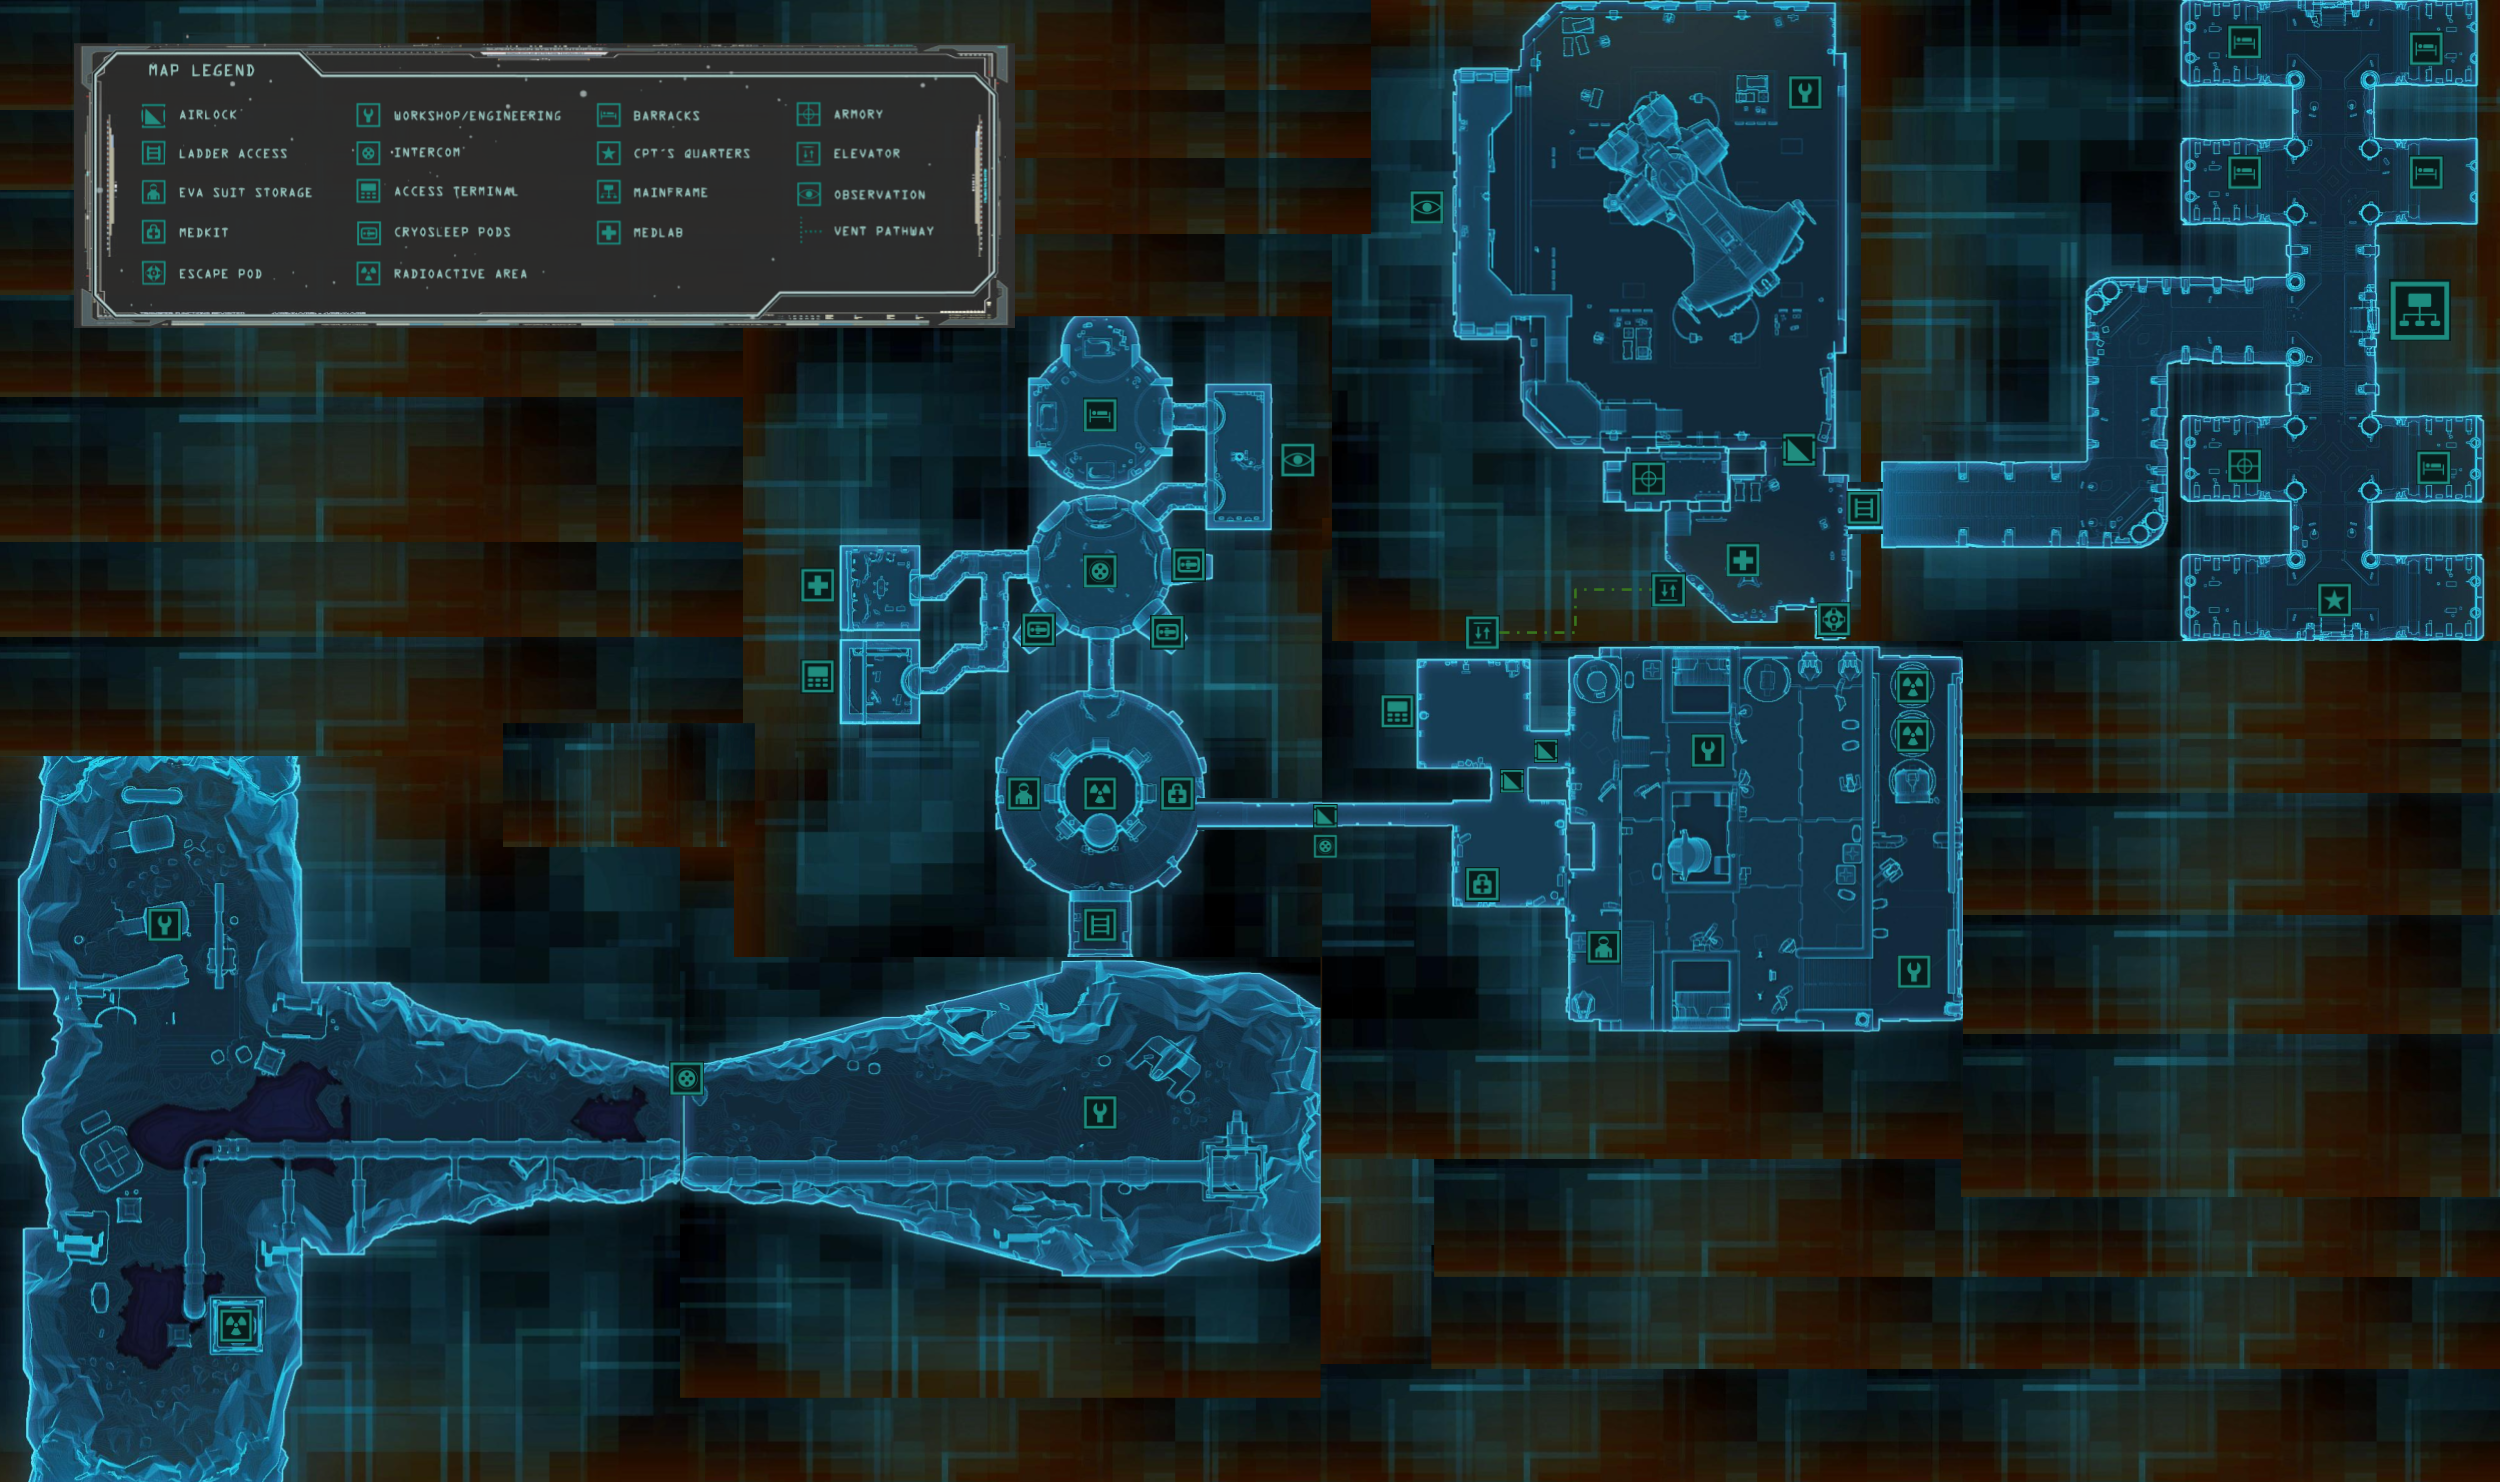
\includegraphics[width=1.05\textwidth]{img/space-refinery-final.png}
    \label{fig:refinery}
\end{sidewaysfigure*}

\newpage
% \chapter{Characters}


\section{Prisoners}


Why the prisoners don't just blow up the place? Well, truth to be told most of them are indeed terrorists and they have plans to either escape, gain control of the station as a new rendezvous point, or take revenge on both United Americas or  Weyland-Yutani. Let's just all accept any plausible excuses and have some fun playing RPG. 



\begin{rpg-pcbox}{Andy Myers}{img/andy.png}
    A drug dealer. You have dwarfism and, over the years, you learned how to use this so that you passed unnoticed through marshals and law enforcement. 
\end{rpg-pcbox}

\begin{rpg-commentbox}{}
    Kid

    \textbf{STRENGTH} 4, \textbf{AGILITY} 4, \textbf{WITS} 2, \textbf{EMPATHY} 4

    \textbf{HEALTH}: 4

    \textbf{SKILLS}: Mobility 3, Medical Aid 1, Observation 1, Manipulation 2
    
    \textbf{TALENT}: dodge
    
    \textbf{GEAR}: IRC MK.50 COMPRESSION SUIT, Radio-controlled cart, Adult magazine
\end{rpg-commentbox}

\newsect

\medskip \medskip \medskip \medskip \medskip \medskip \medskip \medskip \medskip \medskip \medskip \medskip \medskip \medskip \medskip \medskip \medskip \medskip

\begin{rpg-pcbox}{Fredy Cooperr}{img/fredy.png}
    One of the most fearsome terrorists on anchor point station 2. You fought against corporate greed and blew several Weyland-Yutani installations before arrest. 
\end{rpg-pcbox}

\begin{rpg-commentbox}{}
    Officer

    \textbf{STRENGTH} 4, \textbf{AGILITY} 3, \textbf{WITS} 2, \textbf{EMPATHY} 5

    \textbf{HEALTH}: 4

    \textbf{SKILLS}: Ranged Combat 1, Mobility 1, Piloting 2, Observation 1, Medical Aid 1, Command 3, Stamina 1
    
    \textbf{TALENT}: Pull Rank
    
    \textbf{GEAR}: IRC MK.50 COMPRESSION SUIT, Tattoos
\end{rpg-commentbox}

\newsect

\begin{rpg-pcbox}{Jone Heson}{img/jone.png}
    You were wrongly accused for a crime you did not commit. You are a hardworking person and you had hopes that Weyland-Yutani lawyers would reach out and save you. Until then, you have to blend in and survive.
\end{rpg-pcbox}

\begin{rpg-commentbox}{}
    roughneck

    \textbf{STRENGTH} 5, \textbf{AGILITY} 3, \textbf{WITS} 2, \textbf{EMPATHY} 4

    \textbf{HEALTH}: 5

    \textbf{SKILLS}: Heavy Machinery 3, Combat 2, Stamina 2, Observation 1, Survival 1, Comtech 1
    
    \textbf{TALENT}: True Grit, MECHANICAL CUTTING TORCH, Family photo
    
    \textbf{GEAR}: IRC MK.50 COMPRESSION SUIT
\end{rpg-commentbox}

\newsect


\begin{rpg-pcbox}{Ivan Beschastnikh}{img/ivan.png}
    ``dishonorably discharged'' you do not talk about the reason why they threw you in this place either as a punishment worst than death or as a last favor. You are simply ruthless and think that in 3 to 6 months you will be back in the military under some black-ops team.
\end{rpg-pcbox}

\begin{rpg-commentbox}{}
    ex-marine

    \textbf{STRENGTH} 5, \textbf{AGILITY} 3, \textbf{WITS} 2, \textbf{EMPATHY} 3

    \textbf{HEALTH}: 5

    \textbf{SKILLS}: Ranged Combat 3, Mobility 2, Combat 3, Heavy Machinery 1, Command 1
    
    \textbf{TALENT}: Resilient
    
    \textbf{GEAR}: IRC MK.50 COMPRESSION SUIT, hand-made Armat 37A2 12 Shotgun (no ammunition)
\end{rpg-commentbox}

\newsect

\begin{rpg-pcbox}{Hite Chyio}{img/hite.png}
    You were a Yakuza boss. You have blackmail information on several politicians and Weyland-Yutani. Kathia Rison is on her way to get you out of this hell. 
\end{rpg-pcbox}

\begin{rpg-commentbox}{}
    ex-Yakuza

    \textbf{STRENGTH} 2, \textbf{AGILITY} 4, \textbf{WITS} 3, \textbf{EMPATHY} 5

    \textbf{HEALTH}: 2

    \textbf{SKILLS}: Manipulation 3, Comtech 2, Observation 2, Stamina 2, Ranged Combat 1, Mobility 2
    
    \textbf{TALENT}: Personal Safety, Plastic glasses
    
    \textbf{GEAR}: IRC MK.50 COMPRESSION SUIT
\end{rpg-commentbox}


\newsect

\medskip \medskip \medskip \medskip \medskip  \medskip \medskip \medskip \medskip \medskip \medskip \medskip \medskip \medskip \medskip  \medskip \medskip \medskip \medskip \medskip 

\begin{rpg-pcbox}{Henrique Santiago}{img/henrique.png}
    You trafficked people for organs extraction. It suffices to say that your lack any moral restraints.
    Inside the prison, you pulled some favors so that you could smuggle small items. While your new ``business' has been successful, you are paranoid about being caught by a synthetic
\end{rpg-pcbox}

\begin{rpg-commentbox}{}
    Smuggler

    \textbf{STRENGTH} 2, \textbf{AGILITY} 5, \textbf{WITS} 3, \textbf{EMPATHY} 4

    \textbf{HEALTH}: 2

    \textbf{SKILLS}: Ranged Combat 2, Mobility 2, Piloting 3, Heavy Machinery 1, Observation 2
    
    \textbf{TALENT}: Reckless
    
    \textbf{GEAR}: IRC MK.50 COMPRESSION SUIT, pack of cigarettes
\end{rpg-commentbox}

\newsect

\begin{rpg-pcbox}{Nolan Alder}{img/nolan.png}
    A bio-terrorist. Before being caught, you left a sample of Chemical Agent A0-3959X.91–15 in a hidden stash. You plan to escape and launch a bio attack against anchor point station 2
\end{rpg-pcbox}

\begin{rpg-commentbox}{}
    Scientist

    \textbf{STRENGTH} 2, \textbf{AGILITY} 3, \textbf{WITS} 5, \textbf{EMPATHY} 4

    \textbf{HEALTH}: 2

    \textbf{SKILLS}: Mobility 1, Stamina 1, Observation 3, Comtech 2, Manipulation 2, Medical Aid 3
    
    \textbf{TALENT}: Analysis
    
    \textbf{GEAR}: IRC MK.50 COMPRESSION SUIT, M314 Motion Tracker, Blackmail data
\end{rpg-commentbox}


\clearpage

\subsection{Personal Agendas}


 
\begin{rpg-commentbox}{Andy Myers the drug dealer}
    \begin{enumerate}[label=\textbf{Act \arabic*}, leftmargin=1cm]
        \item Sell drugs from his personal stash to two inmates
        \item Find and convince someone to protect him
        \item Grab medical drugs to make his stress decrease
    \end{enumerate}
\end{rpg-commentbox}

\begin{rpg-commentbox}{Fredy Cooperr the terrorist}
    \begin{enumerate}[label=\textbf{Act \arabic*}, leftmargin=1cm]
        \item Make sure the other prisoners acknowledge his command
        \item Grab one land mine for his own personal usage
        \item Kill the marshal
    \end{enumerate}
\end{rpg-commentbox}


\begin{rpg-commentbox}{Henrique Santiago the smuggler}
    \begin{enumerate}[label=\textbf{Act \arabic*}, leftmargin=1cm]
        \item Grab smuggling supplies from one of the guard officers
        \item Make some improvised weapon powerful enough to kill the alien
        \item Get to the ship
    \end{enumerate}
\end{rpg-commentbox}

\begin{rpg-commentbox}{Hite Chyio the Yakuza boss}
    \begin{enumerate}[label=\textbf{Act \arabic*}, leftmargin=1cm]
        \item Discover that Kathia is there to rescue him
        \item Discover hidden camera on Tery
        \item Grab data from hidden camera for personal usage
    \end{enumerate}
    
\end{rpg-commentbox}

\begin{rpg-commentbox}{Ivan Beschastnikh the ex-soldier}
    \begin{enumerate}[label=\textbf{Act \arabic*}, leftmargin=1cm]
        \item Get enough nails to load his improvised shotgun
        \item Make sure Kathia survives
        \item Grab a fucking heavy-weapon
    \end{enumerate}
\end{rpg-commentbox}

\begin{rpg-commentbox}{Jone Heson the roughneck}
    \begin{enumerate}[label=\textbf{Act \arabic*}, leftmargin=1cm]
        \item Protect X from other prisoners
        \item Make some improvised weapon powerful enough to kill the alien
        \item Get to the ship
    \end{enumerate}
\end{rpg-commentbox}

\begin{rpg-commentbox}{Nolan Alder the  bio terrorist}
    \begin{enumerate}[label=\textbf{Act \arabic*}, leftmargin=1cm]
        \item Steal some of the medical supplies from the crew medic
        \item Discover the alien weakness
        \item Grab some of the spores from the Praetorian
    \end{enumerate}
\end{rpg-commentbox}

 
\begin{rpg-commentbox}{The undercover synthetic}
    Change one of the PC agendas by this one. While undercover, the synthetic uses the same attributes as a normal character.

    \begin{enumerate}[label=\textbf{Act \arabic*}, leftmargin=1cm]
        \item Get someone to confess a crime
        \item Get hit and survive a stage II alien attack (potentially capturing a spore within you)
        \item Change the flight plans in the main frame to get you to Weyland-Yutani space
    \end{enumerate}
\end{rpg-commentbox}



\clearpage


\section{Lasalle Bionational crew}

Disguised as Weyland-Yutani annual inspection crew, the Lasalle plans to rescue one of the prisoners who has valuable information against their competitors.


\begin{rpg-pcbox}{Aleki Bowman}{img/bowman.png}
    Chief of security of the Lasalle Bionational crew. You served for many years as a colonial marine, though you noticed that you were a pawn in the corporate/governmental chess match.
\end{rpg-pcbox}

\begin{rpg-commentbox}{}
    mercenary

    \textbf{STRENGTH} 3, \textbf{AGILITY} 5, \textbf{WITS} 2, \textbf{EMPATHY} 3

    \textbf{HEALTH}: 3

    \textbf{SKILLS}: Ranged Combat 2, Mobility 2, Piloting 1, Command 2, Manipulation 1, Combat 1
    
    \textbf{TALENT}: Overkill
    
    \textbf{GEAR}: Armat M41A Pulse Rifle (geo-locked), M3 PERSONNEL ARMOR, dog tag
\end{rpg-commentbox}

\newsect

\begin{rpg-pcbox}{Barby Lopez}{img/lopez.png}
    you brought Kathia on her corporate mission though you know the fame of Kohru and had you had the opportunity, you wouldn't think twice about shutting down the place
\end{rpg-pcbox}

\begin{rpg-commentbox}{}
    pilot

    \textbf{STRENGTH} 4, \textbf{AGILITY} 3, \textbf{WITS} 2, \textbf{EMPATHY} 5

    \textbf{HEALTH}: 4

    \textbf{SKILLS}: Ranged Combat 1, Combat 1, Heavy Machinery 1, Mobility 1, Piloting 2, Observation 1, Stamina 1, Manipulation 1, Comtech 1, Survival 1, Command 1
    
    \textbf{TALENT}: Fast Reflexes
    
    \textbf{GEAR}: .357 Magnum Revolver (2 reloads)
\end{rpg-commentbox}


\newsect

\medskip \medskip \medskip \medskip


\begin{rpg-pcbox}{Kathia Rison}{img/kathia.png}
    On your way to extract Hite from Kohru and get the hell out of this god forsaken place.
    You are arrogant and will always pull your corporate status to get out of messy situations.
\end{rpg-pcbox}

\begin{rpg-commentbox}{}
    Company agent

    \textbf{STRENGTH} 2, \textbf{AGILITY} 3, \textbf{WITS} 4, \textbf{EMPATHY} 4

    \textbf{HEALTH}: 2

    \textbf{SKILLS}: Ranged Combat 2, Mobility 1, Medical Aid 1, Manipulation 3, Observation 2, Comtech 1, Command 3
    
    \textbf{TALENT}: Personal Safety
    
    \textbf{GEAR}: Hairpin
\end{rpg-commentbox}


\newsect

\begin{rpg-pcbox}{Tery Marte}{img/tery.png}
    An activist, you have a hidden camera in your right arm and you falsified paperwork to present yourself as a psychologist. You plan to evaluate the prisoners as an excuse to get first hand data on Kohru and use that for blackmailing or to shut the place down
\end{rpg-pcbox}

\begin{rpg-commentbox}{}
    Roughneck reporter

    \textbf{STRENGTH} 3, \textbf{AGILITY} 3, \textbf{WITS} 4, \textbf{EMPATHY} 4

    \textbf{HEALTH}: 3

    \textbf{SKILLS}: Stamina 2, Survival 1, Comtech 3, Manipulation 2, Medical Aid 2, Mobility 2
    
    \textbf{TALENT}: The long haul
    
    \textbf{GEAR}: Digital Camera
\end{rpg-commentbox}


\clearpage

\subsection{Personal Agendas}

\begin{rpg-commentbox}{Kathia Rison the company agent}
    \begin{enumerate}[label=\textbf{Act \arabic*}, leftmargin=1cm]
        \item Make sure Mageed and the others believe your crew works for Lasalle
        \item Survive
        \item Change the flight plans in the main frame to get you to terrorist space
    \end{enumerate}
    
\end{rpg-commentbox}


\begin{rpg-commentbox}{Tery Marte the reporter}
    \begin{enumerate}[label=\textbf{Act \arabic*}, leftmargin=1cm]
        \item Record prisoner struggles \textbf{requires one mobility and one comtech roll}
        \item Record alien \textbf{requires two slow actions}
        \item Make sure records are released somehow
    \end{enumerate}
\end{rpg-commentbox}



\begin{rpg-commentbox}{Barby Lopez the pilot}
    Change one of the PC agendas by this one. While undercover, the synthetic uses the same attributes as a normal character.

    \begin{enumerate}[label=\textbf{Act \arabic*}, leftmargin=1cm]
        \item Mingle with the crew, making them confess something illegal that happened in the facility
        \item Make the refinery reactor overheat. The station will ultimately explode after T-minus 1 hour
        \item Get back to the ship
    \end{enumerate}
\end{rpg-commentbox}


\begin{rpg-commentbox}{Aleki the mercenary}
    Change one of the PC agendas by this one. While undercover, the synthetic uses the same attributes as a normal character.

    \begin{enumerate}[label=\textbf{Act \arabic*}, leftmargin=1cm]
        \item Assert that no one threatens Kathia
        \item Make sure Hite stays alive
        \item Get heavy weapons in the weapon-locker
    \end{enumerate}
\end{rpg-commentbox}


\clearpage




\section{Kohru crew}


\begin{rpg-pcbox}{Joyce Anderson}{img/joyce.png}
    The chief engineer of the station. This was supposed to be an one-year temporary job. One year turned into two, then into five. You would love to see the place collapse and get a job somewhere safer.
\end{rpg-pcbox}

\begin{rpg-commentbox}{}
    Roughneck

    \textbf{STRENGTH} 5, \textbf{AGILITY} 4, \textbf{WITS} 3, \textbf{EMPATHY} 2

    \textbf{HEALTH}: 5

    \textbf{SKILLS}: Ranged Combat 1, Mobility 1, Medical Aid 1, Heavy Machinery 3, Comtech 2, Survival 1, Stamina 1
    
    \textbf{TALENT}: Resilient
    
    \textbf{GEAR}: IRC MK.50 COMPRESSION SUIT, Electronic tools, Soldering googles
\end{rpg-commentbox}

\newsect

\begin{rpg-pcbox}{Victor Macbeth}{img/victor.png}
    Chief medic on the station. You live for your job and you actually believe in redemption. You decided to work at this place by choice and all the prisoners seem to understand that. If one person can walk freely in the prison block, that person is you.
\end{rpg-pcbox}

\begin{rpg-commentbox}{}
    Medic

    \textbf{STRENGTH} 2, \textbf{AGILITY} 3, \textbf{WITS} 5, \textbf{EMPATHY} 4

    \textbf{HEALTH}: 2

    \textbf{SKILLS}: Stamina 1, Observation 2, Comtech 3, Manipulation 1, Medical Aid 3, Mobility 1, Combat 1
    
    \textbf{TALENT}: Compassion
    
    \textbf{GEAR}: IRC MK.50 COMPRESSION SUIT, SURGICAL KIT, Stethoscope
\end{rpg-commentbox}


\newsect

\medskip \medskip \medskip \medskip \medskip \medskip \medskip \medskip


\begin{rpg-pcbox}{Abdul Mageed}{img/mageed.png}
    A pragmatic. You run the entire station making sure that prisoners don't kill each other (more than the necessary to blow steam off). You turn a blind-eye to people wrongly accused thinking that the few false positives justify all the greater good.
\end{rpg-pcbox}

\begin{rpg-commentbox}{}
    Colonial marshal

    \textbf{STRENGTH} 3, \textbf{AGILITY} 2, \textbf{WITS} 4, \textbf{EMPATHY} 5

    \textbf{HEALTH}: 3

    \textbf{SKILLS}: Ranged Combat 1, Mobility 1, Manipulation 2, Command 3, Comtech 1, Observation 2
    
    \textbf{TALENT}: Nerves of Steel
    
    \textbf{GEAR}: M3 PERSONNEL ARMOR, .357 Magnum Revolver, Station blueprint
\end{rpg-commentbox}


\newsect

\begin{rpg-pcbox}{Mik Elson}{img/mik.png}
    Chief of security. You hate your job. You are trapped in this living hell with some of the worst scum of the sector. You would sacrifice each and every one for your personal survival.
\end{rpg-pcbox}

\begin{rpg-commentbox}{}
    Marine

    \textbf{STRENGTH} 4, \textbf{AGILITY} 4, \textbf{WITS} 2, \textbf{EMPATHY} 3

    \textbf{HEALTH}: 4

    \textbf{SKILLS}: Ranged Combat 2, Mobility 2, Piloting 1, Command 2, Manipulation 1, Combat 1
    
    \textbf{TALENT}: Overkill
    
    \textbf{GEAR}: Armat M41A Pulse Rifle (geo-locked), M3 PERSONNEL ARMOR, dog tag
\end{rpg-commentbox}

\newsect




% \begin{rpg-commentbox}{Joyce Ardson}
%     roughneck: 
% \end{rpg-commentbox}

% \begin{rpg-commentbox}{}
%     medic: 
% \end{rpg-commentbox}

% \begin{rpg-commentbox}{}
%     marine: 
% \end{rpg-commentbox}

% \begin{rpg-commentbox}{Abdul Mageed}
%     : 
% \end{rpg-commentbox}




% \section{NPCs}

% In case you need sidekicks.

% \begin{rpg-commentbox}{random prisoners}
%     \begin{itemize}
%         \item Mito Yoran
%         \item Edzuk Shiro
%         \item Bomba Andres
%         \item Edison Harcrow
%         \item Brom Tower
%         \item Delphine Ryant
%     \end{itemize}

% \end{rpg-commentbox}


% \begin{rpg-commentbox}{Random staff}
%     \begin{itemize}
%         \item Aleve Miroste
%         \item Psycho Dante
%         \item West Nylund
%         \item Jocasta Belmont
%         \item Geneva Macbeth
%         \item Monte Jann
%         \item Hawthorne Thoran
%         \item Harrison Woldt
%     \end{itemize}

% \end{rpg-commentbox}

% \newsect

% \input{sections/act-1}
% \chapter{Act II}




\section{Where the hell is the body?}


\begin{rpg-commentbox}{The Alien}
   The creature controls the host to seek a dark and quiet place where it can grow stronger.

    On its path, it will infect two more prisoners (NPCs) making a larva exo-parasite grow on the host's stomach. 
    The larva are in stealth mode and they need to infect a new host to reach stage II.

    \medskip

    If the PCs had killed the first alien, just have some other prisoners infected and describe gore bodies as they walk through the refinery
\end{rpg-commentbox}


\newsect

\section{Escape plan}


\begin{rpg-commentbox}{Protect Kathia}
    Ideally, Kathia has left her corporate card in a biometric safe, so her protection is paramount to any escape plan.

    Mageed contacts prisoners via intercom and says that the crew is working on a escape plan. They will use Kathia's ship and for that, they need to bypass the lockdown.
    Prisoners are asked to gather enough mining explosives and bring them to the reactor core at the refinery. A handful of explosives can damage the reactor and cut power in the station, that will deactivate the lockdown. However, prisoners will need EVA suits as the air in the station will soon deplenish.
 \end{rpg-commentbox}


 \begin{rpg-commentbox}{Grab Explosives at the mine}
    Depending how players go fetch the mining explosives, they will face the alien fully morphed to stage 2. \textbf{Alien has stats of a Xenomorph stalker}

    Run a stealth mode scene moving some of the players through the mines. \textbf{mobility} vs \textbf{observation}
 \end{rpg-commentbox}


 
 \begin{rpg-commentbox}{Bring explosives to reactor}
    At this point in time, if one of the larva is still alive and the PCs did not encounter it, people will hear agonizing screams as the larva infects a new host. 

    Something cool for this one is to let the host have a welding torch. The alien won't use it but it hangs in a loosely held bandoleer making a lot of noise while the exo-parasite walks the refinery. This can make for some interesting scenes as for example, players setting the explosives in the reactor core while listening to the crackling sound of metal against the crate floor.

    Players must hack the reactor door \textbf{comtech}, put the explosives and set a controlled explosion \textbf{??} Failures might bring nice complications
 \end{rpg-commentbox}

 \begin{rpg-commentbox}{Load cargo elevator with sulfuric acid}
    Needed to crack safe open without corrupting the corporate card

    Players must use crane to pick acid containers \textbf{heavy machinery}
 \end{rpg-commentbox}


 \begin{rpg-commentbox}{Other option}
   Other option is to switch the strategy, use sulfuric acid to open a pathway to the upper level and the mines for opening the hangar hatch.
\end{rpg-commentbox}

 \newsect

 \section{What is happening upstairs?}
 
\begin{rpg-commentbox}{We've got a situation here}
   From time to time Mageed gets in the intercom and give instructions. At some point, let him say hang-on, we got a situation here. All communications after this only return hiss static. Increase stress level by 1.
\end{rpg-commentbox}
% \chapter{Act III}





\begin{rpg-commentbox}{}
    
    Things upstair might have gone south. Even though the crew has side-arms, and a weapons-locker, the creature over took them by surprise. In fact, the alien at this act is at its full potential, stage III. \textbf{Alien has stats of a Xenomorph Praetorian. Reroll 1s as it doesn't have call the guard but keep 2s roll.}

\end{rpg-commentbox}    



\section{War zone}


\begin{rpg-commentbox}{Let's get the hell out of here}
   The PCs must fetch the corporate card at the safe on the crew quarters. \textbf{mobility} vs \textbf{observation}

   When they reach the safe, they discover that it has been cracked open and the card is not there.

   \medskip

    The players might also want to grab side arms or heavy weapons at the weapons locker. For the heavy weapons, they need Mageed's card.
    Mageed is not found anywhere.
\end{rpg-commentbox}



\begin{rpg-commentbox}{What happened here?}
    If players decide to view the logs in the mainframe, they discover that part of the crew has locked themselves in the space shuttle and are waiting 
    for the prisoners to blow the hatch so they can escape instead. \textbf{manipulation} \textbf{command}

    There has to be something in favor of the players, e.g., all pilots are dead and the only person with piloting skills is among the players or in desperation to escape the crew forgot to open some magnetic grips attached to the ship due to security protocols. \textbf{heavy machinery}

    Make all negotiations stressful while the alien havocs the hangar. If players take too long, the Praetorian will produce exo-parasites and drop them on the station so they can hunt new hosts.
 \end{rpg-commentbox}

 
\begin{rpg-commentbox}{Do we really need to kill this thing?}
    Players may get clever and crawl through the ducts and put an explosive on the hangar door sucking the air of the station and the alien. 
    
    Use some of the heavy weapons and diversions to not confront the creature directly, etc.

    Reward clever thinking but punish time lost if decisions are not made fast enough
 \end{rpg-commentbox}

\newsect 

\section{Epilogue} 
 
\begin{rpg-commentbox}{}


\begin{itemize}
    \item Will Lasalle send a crew to gather alien DNA before word spreads out?
    \item Will the reporter release footage of his recordings or blackmail someone?
    \item Do the prisoners take control of the ship or are they out-matched by the surviving crew?
\end{itemize}    

    \medskip

    \textbf{Narrate the epilogue and thank everyone for their time.}
    \end{rpg-commentbox}

    \newsect

    
% % \chapter{Alien}





% \section{Kohru crew}

% \begin{rpg-commentbox}{Joyce Ardson}
%     roughneck: the chief engineer of the station
% \end{rpg-commentbox}

% \begin{rpg-commentbox}{Victor Macbeth}
%     medic: chief medic on the station
% \end{rpg-commentbox}

% \begin{rpg-commentbox}{Mik Elson}
%     marine: chief of security 
% \end{rpg-commentbox}

% \begin{rpg-commentbox}{Abdul Mageed}
%     colonial marshal: a pragmatic. You run the entire station making sure that prisoners don't kill each other (more than the necessary to blow steam off). You turn a blind-eye to people wrongly accused thinking that the few false positives justify all the greater good.
% \end{rpg-commentbox}
% \chapter{Appendix}


\section{Exo-Spore}


\section{Exo-parasite}


\begin{rpg-commentbox}{}

    \centering{\textbf{Stats}}

    \par\noindent\rule{\textwidth}{0.4pt}

    \textbf{SPEED} 2

    \textbf{HEALTH}: 2

    \textbf{SKILLS}: Mobility 8, Observation 8
    
    \textbf{ARMOR}: 2 (0 vs fire)
    
    \textbf{ACID SPLASH}: 4

    \par\noindent\rule{\textwidth}{0.4pt}


    \begin{enumerate}
        \item SKITTERING MENACE The Facehugger has chosen its host and they know it is coming for
        them! It skitters forward, single-minded and horrifyingly spider-like. The victim suffers +1
        STRESS LEVEL and must make an immediate Panic Roll.
        \item same as above
        
        \par\noindent\rule{.9\textwidth}{0.4pt}

        \item TAIL LASH The little monster comes for its target, lashing out with its wicked tail. It attacks
        with five Base Dice, Damage 1.

        \par\noindent\rule{.9\textwidth}{0.4pt}

        \item TAIL GRAPPLE: The Facehugger leaps and catches its victim from behind, its tail whipping
        violently. Roll a D6:
            1–2: The target’s legs are caught and they fall prone—make a Panic Roll.
            
            3–4: The victim’s arms get hopelessly tangled in the beast’s tail—they cannot use any held items and must make a Panic Roll.
            
            5–6: The Facehugger wraps its tail around the target’s neck, choking them—they suffer the effects of DROWNING and must make a Panic Roll. 

        \par\noindent\rule{.9\textwidth}{0.4pt}

        \item SPINE GRAPPLE The Facehugger leaps at its victim. Make an opposed roll with six Base Dice
        against the target’s CLOSE COMBAT skill (not counting as an action for the victim):
            If the Facehugger wins, the target will suffer THE FINAL EMBRACE (below) on the Facehugger’s next initiative.

            If the victim wins they throw the beast to the floor, but it’s not finished with them
        yet and attacks the same target again on its next initiative. 

        \par\noindent\rule{.9\textwidth}{0.4pt}

        \item THE FINAL EMBRACE The Facehugger gets to its victim, its acid making short work of any helmet or respirator in the way. Roll for the attack with six Base Dice. If it gets one or more ,
        the poor victim is facehugged and immediately Broken.
    \end{enumerate}

\end{rpg-commentbox}


\begin{figure}
    \centering
    \includegraphics[width=.45\textwidth]{img/stage-I-bg.png}
    \label{fig:stage-1}
    \caption*{Stage I - Exo-parasite}
\end{figure}

\clearpage

\section{Exo-host}

\begin{figure}
    \centering
    \includegraphics[width=.45\textwidth]{img/stage-II-bg.png}
    \label{fig:stage-2}
    \caption*{Stage II - Exo-host}
\end{figure}


\clearpage

\section{Exo-alien}

\begin{figure}
    \centering
    \includegraphics[width=\textwidth]{img/stage-III-bg.png}
    \label{fig:stage-3}
    \caption*{Stage III - Exo-alien}
\end{figure}

% End document
\end{document}
